%%%%%%%%%%%%%%%%%%%%%%%%%%% asme2ej.tex %%%%%%%%%%%%%%%%%%%%%%%%%%%%%%%
% Template for producing ASME-format journal articles using LaTeX    %
% Written by   Harry H. Cheng, Professor and Director                %
%              Integration Engineering Laboratory                    %
%              Department of Mechanical and Aeronautical Engineering %
%              University of California                              %
%              Davis, CA 95616                                       %
%              Tel: (530) 752-5020 (office)                          %
%                   (530) 752-1028 (lab)                             %
%              Fax: (530) 752-4158                                   %
%              Email: hhcheng@ucdavis.edu                            %
%              WWW:   http://iel.ucdavis.edu/people/cheng.html       %
%              May 7, 1994                                           %
% Modified: February 16, 2001 by Harry H. Cheng                      %
% Modified: January  01, 2003 by Geoffrey R. Shiflett                %
% Use at your own risk, send complaints to /dev/null                 %
%%%%%%%%%%%%%%%%%%%%%%%%%%%%%%%%%%%%%%%%%%%%%%%%%%%%%%%%%%%%%%%%%%%%%%

%%% use twocolumn and 10pt options with the asme2ej format
\documentclass[twocolumn,10pt]{asme2ej}

\usepackage{amsmath}
\usepackage{amsfonts}
\usepackage{graphicx}

\usepackage{algorithms}
\usepackage{algorithmic}
\renewcommand{\algorithmicrequire}{\textbf{Input:}}
\renewcommand{\algorithmicensure}{\textbf{Output:}}

%\makeatletter
%\newif\if@restonecol
%\makeatother
%\let\algorithm\relax
%\let\endalgorithm\relax
%\usepackage{algorithm2e}

\usepackage[colorlinks]{hyperref}
%\usepackage[colorinlistoftodos, textwidth=4cm, shadow]{todonotes}

\let\Omin\minute
\let\minute\undefined

\let\Ohour\hour
\let\hour\undefined

\usepackage{siunitx}

\newcommand{\etal}{et al.}
%%\usepackage{psfig} %% for loading postscript figures

%% The class has several options
%  onecolumn/twocolumn - format for one or two columns per page
%  10pt/11pt/12pt - use 10, 11, or 12 point font
%  oneside/twoside - format for oneside/twosided printing
%  final/draft - format for final/draft copy
%  cleanfoot - take out copyright info in footer leave page number
%  cleanhead - take out the conference banner on the title page
%  titlepage/notitlepage - put in titlepage or leave out titlepage
%  
%% The default is oneside, onecolumn, 10pt, final


\title{Speeding Up Particle Trajectory Simulations under Moving Force Fields using GPUs}


%%% first author
\author{ Robert Patro
    \affiliation{
	Graduate Student\\
	Inst. for Advanced Computer Studies\\
	Department of Computer Science\\
	University of Maryland\\
	College Park, Maryland 20742\\
    Email: rob@cs.umd.edu
    }	
}

%%% second author
\author{ John P. Dickerson
    \affiliation{
	Research Assistant\\
	Inst. for Advanced Computer Studies\\
	University of Maryland\\
	College Park, Maryland 20742\\
    Email: johnd@umiacs.umd.edu
    }	
}

%%% third author
\author{ Sujal Bista
  \affiliation{
    Graduate Student\\
    Inst. for Advanced Computer Studies\\
    Department of Computer Science\\
    University of Maryland\\
    College Park, Maryland 2072\\
    Email: sujal@cs.umd.edu
  }  
}
%%% fourth author
\author{ Satyandra K. Gupta
   \affiliation{ Professor, Fellow of ASME\\
	Inst. for Systems Research\\
	Department of Mechanical Engineering\\
	University of Maryland\\
	College Park, Maryland 20742\\
   Email: skgupta@umd.edu
   }
}

%%% fifth author
\author{ Amitabh Varshney
    \affiliation{ Professor\\
	Inst. for Advanced Computer Studies\\
	Department of Computer Science\\
	University of Maryland\\
	College Park, Maryland 20742\\
    Email: varshney@cs.umd.edu
    }
}



\begin{document}

\maketitle    

%%%%%%%%%%%%%%%%%%%%%%%%%%%%%%%%%%%%%%%%%%%%%%%%%%%%%%%%%%%%%%%%%%%%%%
\begin{abstract}

  In this paper, we introduce a GPU-based framework for simulating particle trajectories under both static and dynamic force fields.  By exploiting the highly parallel nature of the problem and making efficient use of the available hardware, our simulator exhibits a significant speedup over its CPU-based analog.  We apply our framework to a specific experimental simulation: the computation of trapping probabilities associated with micron-sized silica beads in optical trapping workbenches.  When evaluating large numbers of trajectories ($4096$), we see approximately a $356$ times speedup of the GPU-based simulator over its CPU-based counterpart.

\end{abstract}

%%%%%%%%%%%%%%%%%%%%%%%%%%%%%%%%%%%%%%%%%%%%%%%%%%%%%%%%%%%%%%%%%%%%%%
%\begin{nomenclature}
%\entry{A}{You may include nomenclature here.}
%\entry{$\alpha$}{There are two arguments for each entry of the nomemclature
%environment, the symbol and the definition.}
%\end{nomenclature}
%
%%%%%%%%%%%%%%%%%%%%%%%%%%%%%%%%%%%%%%%%%%%%%%%%%%%%%%%%%%%%%%%%%%%%%%

%% S.K.ized intro
\section{Introduction}

The simulation of particle movement under general force fields is of interest
across many scientific disciplines.  For example, biochemists may wish to model
stochastic diffusion of glutamate receptors~\cite{20233407}, while financial
analysts may attempt to simulate point estimates of stock prices based on stochastic
models~\cite{broadie2006exact}.  In this paper, we present a framework to
simulate such general particle movement under user-defined force fields.  We apply this
framework to the task of manipulating micro
and nanoscale components using an optical force field. 

Micro and nanoscale components can be
used to exploit new phenomena that take place at the small scale
~\cite{Bhus04}. Potential applications of such small components include
bio-sensors, electronic components, photonic devices, solar cells, and
batteries~\cite{Niem04,Wils02}.  In order to construct useful devices, micro and nanoscale components need to be
assembled together. Assembling small components to make functional
devices remains a challenge despite rapid advances in imaging,
measurement, and fabrication at the small scale. Two types of assembly
processes are possible at the small scale. The first type of process is
self-assembly~\cite{Requ06}. This process is useful for large scale
production. The second type of process is directed assembly. This
process is useful for prototyping new design concepts, small scale
production, device repair, and creating templates for certain types of
self-assembly processes. In this paper, we limit ourselves to directed
assembly processes. A number of manipulation techniques for directed
assembly of small components have emerged.

In order to manipulate a small component, the appropriate optical,
electrostatic, or magnetic field (i.e., trap) needs to be created to
trap the component. The field is then controlled to move the component. 
In this paper, we focus on the optical force fields and traps associated with them. 
Optical trapping takes place
in a fluidic workspace. The interaction between the optical field and the
component is stochastic in nature, due to the Brownian motion of the
component, as well as the presence of uncertainty in the component location as
a result of sensor errors. Unfortunately, the off-line planning
approach that works well at the macroscale does not work at the
small scale. To cope with the stochastic nature of the problem,
automated microscale assembly requires a real-time and automated
planning paradigm that takes actions based on the estimated state of
the workspace in a feedback loop~\cite{Banerjee:2010:ieee}.

In order to develop automated, real-time planning algorithms, we need
to develop a fundamental understanding of the interaction of
components with trapping fields. For example, we need to
understand and characterize trapping probability, trap reliability,
and trap robustness. The knowledge of the trapping probability will
enable us to position the optical trap close enough to the
component of interest so that it gets trapped. Moreover, any other
component that drifts close enough to the optical trap, such that its
trapping probability exceeds a certain threshold value, is a potential
or imminent source of unintended trapping. Thus, appropriate collision
prevention schemes need to be applied in such cases to avoid losing
the trapped component. Under different operating conditions,
components interact qualitatively differently with the
trap. Unfortunately, the parameter space that describes different
operating conditions is very large. Hence, simulation is the only
viable option for characterizing the interactions between the trap and
the component to facilitate real-time planning.   

This paper presents a GPU-based method to simulate the trajectory of 
particles under a force field. The method described in this
paper is able to handle time varying force fields. The accuracy of
computation depends on the accuracy of the force field. We illustrate
the usefulness of this method by showing how it can be
used to estimate trapping probabilities for moving optical traps. This
new method presents considerable computational improvements over our
previous approach to conducting CPU-based simulations for estimating
trapping probabilities. The work presented in this paper enables fast
computation of trapping probabilities. Faster computation of trapping
probabilities presents three main advantages. First, it enables
exploration of a much larger parameter space. Hence, it improves our
understanding of trapping physics. Second, fast computation of
trapping probabilities eliminates the need for the use of
meta-modeling during the particle transport planning. Finally, faster
computation enables more simulation runs and hence we get better
estimates of the trapping probability.


\section{Related Work}

Since the initial discovery of optical gradient
forces~\cite{ashkin1970acceleration} and subsequent invention of
optical tweezers~\cite{ashkin1986observation}, the use of optical
traps to manipulate micron-sized objects has been widespread.
Simulations of the optical traps play an important role in utilizing
optical tweezers as assembly tools at the micro and nanoscale~\cite{Banerjee:2010:ieee}. Early work in this area focused on
trap and particle interactions and models were developed to estimate
optical forces acting on spherical particles. As a part of our recent
prior work, we developed a model to simulate the trajectory of a
spherical particle under optical forces~\cite{
  banerjee2009generating}. This model was implemented on a CPU and used
to generate trapping probability estimates by conducting off-line
simulations. A meta-model was developed to quickly query trapping
probability estimates during the automated path
planning~\cite{Banerjee:2010:ieee}. CPU-based simulations are very
time consuming. Hence, in an offer to speed up the simulation process,
we successfully implemented Brownian motion simulation on
GPU~\cite{balijepalli2010stochastic}. The current paper builds on our
previous work and presents a new GPU-based method for computing
particle trajectories under optical force fields. In computing
particle trajectories, it combines both the influence of Brownian
motion and an optical force field in a single unified GPU-based
framework.

Graphics processors have evolved over the last decade from a
fixed-function (rendering-only) pipeline to a highly flexible
programmable pipeline.  One of the application areas that has received
significant attention in this evolution has been physically-based
simulations due to their application to simulation of environmental
effects for 3D games~\cite{Owens:2007:ASO}. Some of the earliest work
in this area involved physically-based wave simulations on 2D
lattices~\cite{James:2001:operations}. More general Lattice-Boltzmann
3D simulations for fluids and gases were later implemented on GPUs by
Li et al.~\cite{LWK03,LFWK05}. Other fluid simulations on GPUs include
work on Navier-Stokes equations for incompressible fluids (see review
in this area by Harris~\cite{Harris:2005:fast-fluid}) as well as
Euler-equations-based dynamics of ideal gases (Hagen et
al.~\cite{Hagen:2006:euler}). Work on fluid simulation has also been
extended to deal with
obstacles~\cite{Bolz:2003:sparse,KW03,LLW04,STM04,Harris:2005:fast-fluid}. Visualization
of flows on GPUs has been addressed through line-integral convolution
and Lagrangian-Eulerian
advection~\cite{Heidrich:1999:pixel-textures,JEH01,WHE01}.  Recent
work by Juba and Varshney~\cite{Juba:2008:PSMM} shows the suitability
of the GPUs for stochastic calculations.

%, using Cg and CUDA respectively,
Initial work has been done porting optical trapping simulations to
graphics processors; however, to our knowledge, no GPU-based trapping
probability estimation work exists.  \cite{reicherter:59301Y} and
\cite{haist2006using} simulate the manipulation of glass microspheres
within a holographic laser testbed.  Due to accelerated
two-dimensional FFT calculations, both show significant computational
speedups over their CPU-based counterparts.  Similar results are
available for arbitrarily positioned dual-beam (``twin'')
traps~\cite{hermerschmidt2007holographic}.  Using a model similar to
ours, Balijepalli~\cite{balijepalli2010stochastic} provides an
accuracy and error analysis of results from both CPU and GPU, along
with experimental validation of the simulation.





%%%%%%%%%%%%%%%%%%%%%%%%%%%%%%%%%%%%%%%%%%%%%%%%%%%%%%%%%%%%%%%%%%%%%%
\section{Calculating Trapping Probabilities}
\label{sec:calculating-trapping-probabilities}

Both fully- and semi-autonomous operation of optical tweezers require
the capability to trap a particle and plan its path through the
workspace; avoiding collisions with other components in real-time.
The probability that a given particle will be trapped within a
predictable spatial region about the laser beam focus, or {\em
  trapping probability}, is a critical aspect of this real-time motion
planning problem.  As it is infeasible to determine trapping
probabilities through real-world experiments due to a large parameter
space (including, for example, initial particle position, neighboring
workspace component existence, motion of laser), we have developed a
computational framework in which trapping probabilities can be
determined through optical tweezers simulation.

\subsection{Simulated Particle Motion}
Our initial code operates on glass and silica microspheres, as these are
well-studied in the literature~\cite{wright1994parametric}.  Furthermore,
properties of these spheres can be accurately modeled using theoretically- and
experimentally-verified equations.

In general, any moving component in the workspace will experience hydrodynamic
forces coupled with a rapidly fluctuating force, the result of frequent and
numerous collisions with surrounding liquid molecules.  We can model these
closely connected forces using Langevin's equation~\cite{gardiner1985handbook,
langevin1908brownianmotion}. We use model given in ~\cite{balijepalli2010stochastic}.
Given a velocity $V$, we describe the change in
velocity over time as:
\begin{equation}
\label{eq:langevins-equation}
 \frac{dV(t)}{dt} = -\frac{\gamma}{m}V(t) + \frac{\xi}{m}\Gamma(t)
\end{equation}

The hydrodynamic forces over time ($t$), are a function of velocity
($V$), mass ($m$), and drag ($\gamma$).  The drag coefficient $\gamma$
is given by Stokes' Law~\cite{girault1979finite} as $\gamma = 6 \pi
\eta r$, with $\eta$ representing the fluid viscosity as a function of
temperature and $r$ representing the radius of the silica sphere, in
this case.  The stochastic, rapidly fluctuating force $\Gamma$ is
scaled by a constant $\xi$ satisfying the fluctuation-dissipation
theorem~\cite{weissbluth1989photon}, which is defined as $\xi =
\sqrt{2 \gamma K_B T}$, with $K_B$ representing Boltzmann's
constant~\cite{grassia2001dissipation}.  The stochastic term $\Gamma$
prevents a direct analytic solution to Langevin's equation; as such,
our framework uses a finite difference expression of
Equation~\ref{eq:langevins-equation}.  
The stochastic term $\Gamma$ is substituted by a appropriately scaled normal distribution
$N(0,1/\delta t)$ where $\delta t$ is the finite time step. The term  
$1/\sqrt{\delta t}$ is absorbed into a scaling constant as described in~\cite{balijepalli2010stochastic}.


%The hydrodynamic forces over time ($t$), are a function of velocity
%($V$), mass ($m$), and drag ($\gamma$).  The drag coefficient $\gamma$
%is given by Stokes' Law~\cite{girault1979finite} as $\gamma = 6 \pi
%\eta r$, with $\eta$ representing the fluid viscosity as a function of
%temperature and $r$ representing the radius of the silica sphere, in
%this case.  The stochastic, rapidly fluctuating force $\Gamma$ is
%scaled by a constant $\xi$ satisfying the fluctuation-dissipation
%theorem~\cite{weissbluth1989photon}, which is defined as $\xi =
%\sqrt{2 \gamma K_B T}$, with $K_B$ representing Boltzmann's
%constant~\cite{grassia2001dissipation}.  The stochastic term $\Gamma$
%prevents a direct analytic solution to Langevin's equation; as such,
%our framework uses a finite difference expression of
%Equation~\ref{eq:langevins-equation}.  We substitute a normal
%distribution $N(0,1)$ for $\Gamma$ and alter the scaling constant
%$\xi$ appropriately to include $\delta t$, the finite time step.

We combine the finite difference form of Langevin's equations with an
enumeration of all other forces affecting a silica sphere in the workspace to
yield Equation~\ref{eq:numerical-integration-equation}.  The external force
factor $F_{ext}$ includes the constant (for a sphere) forces of gravity and
buoyancy, as well as the all-important optical trapping force 
applied by the laser to the particle.

%\begin{equation}
%\label{eq:numerical-integration-equation}
% \frac{V(t + \delta t) - V(t)}{\delta t}  = -\frac{\gamma}{m}V(t) + \frac{1}{m}
%\sqrt{\frac{2 \gamma K_B T}{\delta t}} N(0,1) + \frac{F_{ext}}{m} 
%\end{equation}

\begin{equation}
\label{eq:numerical-integration-equation}
 A(t + \delta t)  = -\frac{\gamma}{m}V(t) + \frac{1}{m}
\sqrt{\frac{2 \gamma K_B T}{\delta t}} N(0,1) + \frac{F_{ext}}{m} 
\end{equation}


We explicitly integrate Equation~\ref{eq:numerical-integration-equation}
to obtain a simulation of particle movement over time.  In practice, the most
popular explicit integration techniques include fourth-order Runge-Kutta
methods~\cite{jameson1981numerical}, the Gear predictor-corrector
method~\cite{allen1990computer}, and second-order ``velocity'' Verlet
integration~\cite{verlet1968computer}.  Each is appropriate in certain
situations; as such, we use Verlet integration
(Equations~\ref{eq:velocity-verlet-integration-position}
and~\ref{eq:velocity-verlet-integration-velocity}) due to its conservation of
energy at larger time steps and ease of computation, as discussed
in~\cite{balijepalli2010stochastic}.  Since the time step has a direct effect on
the number of iterations required to run a simulation (and thus its runtime), we
are interested in maximizing time step size while maintaining tight error
bounds.

\begin{equation}
 \label{eq:velocity-verlet-integration-position}
 X(t + \delta t) = X(t) + V(t)\delta t + \frac{1}{2} A(t) \delta t^2 + O(\delta
t^4)
\end{equation}

\begin{equation}
 \label{eq:velocity-verlet-integration-velocity}
 V(t + \delta t) = V(t) + \frac{A(t + \delta t) + A(t)}{2} \delta t + O(\delta
t^2)
\end{equation}

Given velocity $V(t)$ and external force factor $F_{ext}$, we compute the acceleration
$A(t + \delta t )$ at the next time step using
Equation~\ref{eq:numerical-integration-equation}. From here, the
velocity Verlet method provides the next position, $X(t + \delta t)$,
and velocity, $V(t + \delta t)$, in a single pass.


The characteristic time scale of our entire model is given by the
relaxation time $\frac{m}{\gamma}$, with $\gamma = 6 \pi \eta r$ the drag
coefficient of Stokes' equations; this is the time needed for a particle's
initial velocity to converge to thermal equilibrium.  In our experiments, the
numerical integration time step $\delta t$ is set to the nearest multiple of
$100$ ns such that $\delta t << \frac{m}{\gamma}$. Choosing such a small $\delta
t$ provides an opportunity to observe interesting nonequilibrium behavior in the
simulation.  Furthermore, this small time step decreases maximum error in both
velocity and position, bounded by the velocity Verlet to $O(\delta t^2)$ and
$O(\delta t^4)$, respectively.

%\paragraph{Calculation of Force Fields.}
Our particle simulation framework accepts either a continuous or discretely
sampled force field.  In our experiments, we choose to represent the optical
field discretely.  Force values are provided by
numerically integrating the basic scattering and gradient forces of
radiation (see Ashkin's seminal paper~\cite{ashkin1986observation}).  Such
integration is
typically done by tracing representative rays of light from the laser
position through the workspace to the laser focus -- and possibly
through microspheres in the workspace.  By tracing the reflection and
refraction of these simulated rays, a reliable estimate of both the
scattering and gradient forces can be computed.  In our prototype
implementation, we rely on code written
in~\cite{banerjee2009generating} to obtain these forces.

\subsection{Trapping Probability Estimates}

To estimate trapping probabilities, particle trajectory simulation
is performed multiple times at a given point in the parameter
space. The simulation is conducted by starting the particle at the
designated location. The trapping probability is estimated as a ratio
of the number the times the sphere gets trapped by the laser beam over
the total number of trials.

Trapping is a complex phenomenon due to the Brownian motion of the
particles. If a beam is held stationary for an indefinite period of
time, then particles far away from the beam are likely to wander
into the beam due to Brownian motion and eventually be
trapped. Particles continue to exhibit Brownian motion even after they
have been trapped. Therefore, trapped particles eventually jump out of
the trap at practically useful laser powers.  Many different notions
of trapping probability can be defined based on the context. For the
purpose of this paper, we are mainly interested in a notion of
trapping probability which is relevant from the point of view of path
planning. In this application, the laser beam continues to
move. Hence, the time available for trapping is relatively small. For
the purpose of this paper, we have done all trapping probability
estimates for fixed finite period of time. Methodology presented in
this paper can be easily used to compute trapping probability as a
function of the available trapping time.

We have assumed that the Brownian motion inside the trap is
negligible. Hence, the mean time to escape of the trap is quite large
with respect to the planning horizon. Therefore, we do not account for
the possibility of a trapped particle escaping the trap in our
calculations.  The simulation infrastructure has a built-in capability
to simulate Brownian motion under the force field. Therefore, it can
automatically account for the situations where a particle will escape
the trap if the simulation is performed over the long period of time.
For the figures produced in this paper, we assume a particle to be
trapped if the probability of a particle escaping the laser within
$\SI{1}{\deci\second}$ is less than $\frac{1}{N}$, where $N$ is the
number of simulated trajectories per grid position.



%\documentclass{article}
%\begin{document}
%\todo[inline]{How we calculate trapping probabilities and why it's important}

% Both fully- and semi-autonomous operation of optical tweezers require the
% capability to trap a particle and plan its path through the workspace, avoiding
% collisions with other components, in real-time.  The probability that a given
% particle will be trapped within a predictable spatial region about the laser
% beam focus, or {\em trapping probability}, is a critical aspect of this
% real-time motion planning problem.  As it is infeasible to determine trapping
% probabilities through real-world experiments due to a large parameter space
% (including, for example, initial particle position, neighboring workspace
% component existence, motion of laser), we have developed a computational
% framework in which trapping probabilities can be determined through optical
% tweezers simulation.

% \subsection{Simulated Particle Motion}
% Our initial code operates on glass and silica microspheres, as these are
% well-studied in the literature~\cite{wright1994parametric}.  Furthermore,
% properties of these spheres can be accurately modeled using theoretically- and
% experimentally-verified equations.

% In general, any moving component in the workspace will experience hydrodynamic
% forces coupled with a rapidly fluctuating force, the result of frequent and
% numerous collisions with surrounding liquid molecules.  We can model these
% closely connected forces using Langevin's equation~\cite{gardiner1985handbook,
% langevin1908brownianmotion}. Given a velocity $V$, we describe the change in
% velocity over time as:
% \begin{equation}
% \label{eq:langevins-equation}
%  \frac{dV(t)}{dt} = -\frac{\gamma}{m}V(t) + \frac{\xi}{m}\Gamma(t)
% \end{equation}

% The hydrodynamic forces are a function of velocity, mass, and drag.  The drag
% coefficient $\gamma$ is given by Stokes' Law~\cite{girault1979finite} as $\gamma
% = 6 \pi \eta r$, with $\eta$ representing the fluid viscosity as a function of
% temperature and $r$ representing the radius of the silica sphere, in this case. 
% The stochastic, rapidly fluctuating force $\Gamma$ is scaled by a constant $\xi$
% satisfying the fluctuation-dissipation theorem~\cite{weissbluth1989photon},
% which is defined as $\xi = \sqrt{2 \gamma K_B T}$, with $K_B$ representing
% Boltzmann's constant~\cite{grassia2001dissipation}.  The stochastic term
% $\Gamma$ prevents a direct analytic solution to Langevin's equation; as such,
% our framework uses a finite difference expression of
% Equation~\ref{eq:langevins-equation}.  We substitute a normal distribution
% $N(0,1)$ for $\Gamma$ and alter the scaling constant $\xi$ appropriately to
% include $\delta t$, the finite time step.

% We combine the finite difference form of Langevin's equations with an
% enumeration of all other forces affecting a silica sphere in the workspace to
% yield Equation~\ref{eq:numerical-integration-equation}.  The external force
% factor $F_{ext}$ includes the constant (for a sphere) forces of gravity and
% buoyancy, as well as the all-important optical trapping force 
% applied by the laser to the particle.

% \begin{equation}
% \label{eq:numerical-integration-equation}
%  \frac{V(t + \delta t) - V(t)}{\delta t}  = -\frac{\gamma}{m}V(t) + \frac{1}{m}
% \sqrt{\frac{2 \gamma K_B T}{\delta t}} N(0,1) + \frac{F_{ext}}{m} 
% \end{equation}

% We explicitly integrate Equation~\ref{eq:numerical-integration-equation}
% to obtain a simulation of particle movement over time.  In practice, the most
% popular explicit integration techniques include fourth-order Runge-Kutta
% methods~\cite{jameson1981numerical}, the Gear predictor-corrector
% method~\cite{allen1990computer}, and second-order ``velocity'' Verlet
% integration~\cite{verlet1968computer}.  Each is appropriate in certain
% situations; as such, we use Verlet integration
% (Equations~\ref{eq:velocity-verlet-integration-position}
% and~\ref{eq:velocity-verlet-integration-velocity}) due to its conservation of
% energy at larger time steps and ease of computation, as discussed
% in~\cite{balijepalli2010stochastic}.  Since the time step has a direct effect on
% the number of iterations required to run a simulation (and thus its runtime), we
% are interested in maximizing time step size while maintaining tight error
% bounds.

% \begin{equation}
%  \label{eq:velocity-verlet-integration-position}
%  X(t + \delta t) = X(t) + V(t)\delta t + \frac{1}{2} A(t) \delta t^2 + O(\delta
% t^4)
% \end{equation}

% \begin{equation}
%  \label{eq:velocity-verlet-integration-velocity}
%  V(t + \delta t) = V(t) + \frac{A(t + \delta t) + A(t)}{2} \delta t + O(\delta
% t^2)
% \end{equation}

% Given position $X(t)$ and velocity $V(t)$, we compute the
% acceleration $A(t + \delta t )$ at the next time step using
% Equation~\ref{eq:numerical-integration-equation}.  From here, the velocity
% Verlet method provides position $X(t + \delta t)$ and $V(t + \delta t)$ in
% a single pass.

% The characteristic time scale of our entire model is given by the
% relaxation time $\frac{m}{\gamma}$, with $\gamma = 6 \pi \eta r$ the drag
% coefficient of Stokes' equations; this is the time needed for a particle's
% initial velocity to converge to thermal equilibrium.  In our experiments, the
% numerical integration time step $\delta t$ is set to the nearest multiple of
% $100$ ns such that $\delta t << \frac{m}{\gamma}$. Choosing such a small $\delta
% t$ provides opportunity to observe interesting nonequilibrium behavior in the
% simulation.  Furthermore, this small time step decreases maximum error in both
% velocity and position, bounded by the velocity Verlet to $O(\delta t^2)$ and
% $O(\delta t^4)$, respectively.

% \paragraph{Calculation of Optical Trapping Forces.}
% Numerical integration of the basic scattering and gradient forces of radiation (see Ashkin's seminal
% paper~\cite{ashkin1986observation}) yields our desired optical trapping forces.  Such integration is typically done by
% tracing representative rays of light from the laser position through the workspace to the laser focus -- and possibly
% through microspheres in the workspace.  By tracing the reflection and refraction of these simulated rays, a
% reliable estimate of both the scattering and gradient forces can be computed.  In our prototype implementation, we rely
% on code written in~\cite{banerjee2009real} to obtain these forces.

% \subsection{Trapping Probability Estimates}
% S.K. writes about motivation here?

%\end{document}


%%%%%%%%%%%%%%%%%%%%%%%%%%%%%%%%%%%%%%%%%%%%%%%%%%%%%%%%%%%%%%%%%%%%%%
\section{Massively Parallel Simulations}
\label{sec:parallel-simulations}

\begin{figure*}[htb!]
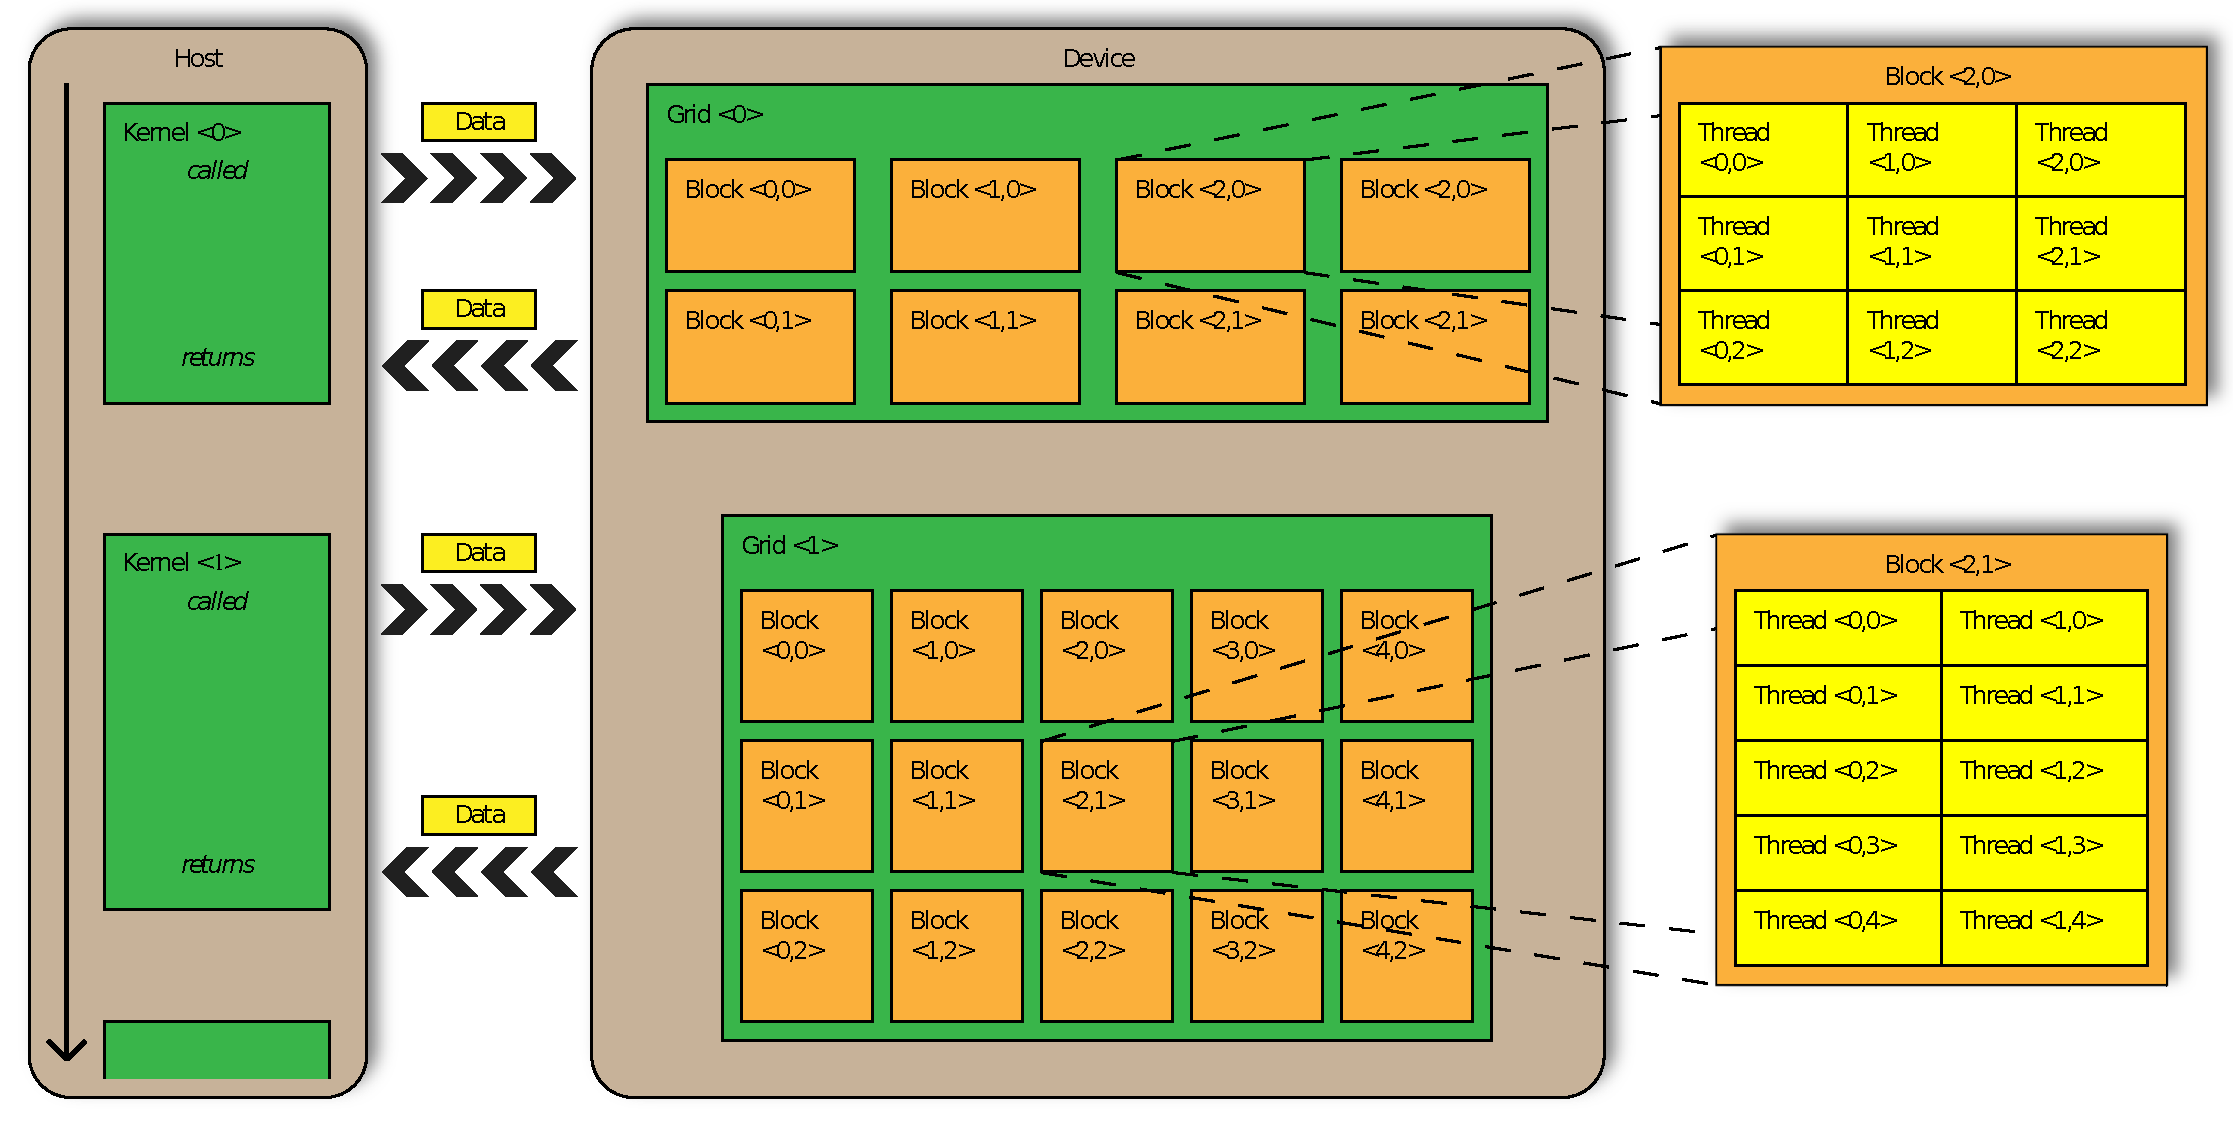
\includegraphics[width=2\columnwidth]{figures/cuda_architecture}
\caption{The CUDA architecture provides for a logical hierarchy of
  parallelism that maps well to the hardware.  The computational
  kernel is run in parallel among a large number of threads which are
  grouped into $1$,$2$ or $3$ dimensional thread blocks.  Threads
  within a block may communicate using the shared memory or coordinate
  execution using synchronization primitives.  The blocks are likewise
  grouped into $1$,$2$ or $3$ dimensional grids.  Each thread is able
  to access its own grid, block and thread identifiers.}
\label{fig:cuda_arch}
\end{figure*}


\subsection{Overview}
\label{sec:parallel-overview}
We leverage the massively parallel architecture of the GPU to expedite
the calculation of trapping probabilities over a wide range of
locations relative to the focal point of the laser.  In particular, we
consider a discrete grid, $G = \{[y_{i},z_{j}]\}$ of particle
locations.  

% Whoops, this is the force texture, not the evaluation grid 

% In all of our experiments, we consider
% $\SI{0}{\micro\meter} \le y_{i} \le \SI{20}{\micro\meter}$ and
% $\SI{-20}{\micro\meter} \le z_{i} \le \SI{8}{\micro\meter}$, leading
% to a total of $560$ grid cells at which the trapping probability needs
% to be evalutated. 

As detailed in section~\ref{sec:calculating-trapping-probabilities},
the particles we are interested in trapping undergo motion governed
by the Langevin equation; which contains a stochastic component
modeling the Brownian motion of the particles.  Thus, a reliable
estimate of the trapping probability at a particular grid cell,
$[y,z]$, can only be obtained by repeatedly simulating the trajectory
of a particle intially placed at $[y,z]$.  To obtain a $95\%$
confidence interval of less than $\pm 0.03125$ on our estimated trapping probability, we 
simulate the particle trajectories $1024$ times at each grid cell.  The
greater the degree of confidence we require, the more trajectories we
must simulate for each cell on the simulation grid $G$.  This is a
highly computationally intensive, but inherently parallel process.  In
particular, the estimation of the trapping probability at each grid
cell can be done independently.

Though the parallel nature of the problem is straightforward,
consideration is still required if we are to achieve optimal
performance on current hardware.  In all of the experiments detailed
below, we have performed the trapping probability estimates on an
Nvidia Tesla S1070; a GPU computing oriented, CUDA capable device.  A
diagram of the CUDA architecture -- how the threads of execution and
memory are arranged -- is provided in Figure~\ref{fig:cuda_arch}.

\paragraph{GPU vs. CPU implementations}
While this paper focuses on a GPU implemetation of the trapping
probability calculation, we wish to draw attention to the fact that it
is the massively parallel nature of this computation, and not the
specific GPU implementation, that is of the broadest interest.  In
particular, the CPU implementation with which we contrast our GPU
implementation, while reasonably efficient, still has many avenues for
optimization.  Specifically, we compare GPU performance against a
single-threaded CPU implementaion that does not take advantage of
vectorized instructions.  While it is certainly true that the CPU
implemenation could be improved to offer better performance, the most
important observation is the rate at which the simulation results
scale.  Since each simulation can be performed independently, the
overall computation of trapping probabilities is massively data
parallel.  Thus, while the performance gap between the two
implementations can undoubtedly be shrunken somewhat, the
data-parallel nature of the problem ensures that scalable parallel
architecture of the GPU will continue to provide a very significant
benefit.

\subsection{Data Structures}
\label{sec:data-structures}

There are two obvious was to parallelize the computation of trapping
probabilities: among grid cells or among particles.  We choose the
latter of these two as we feel it offers more flexiblity and
allows us to maximally utilize the GPU.  There are four major sources
of input to the simulation kernel:

\begin{enumerate}
\item an array of particles
\item a force grid
\item a set of fundamental physical constants
\item a stream of pseudorandom numbers
\end{enumerate}

Care must be taken to ensure that each of these input sources is
amenable to GPU computation.  Each particle maintains a position,
velocity, acceleration, and state variable.  The position, velocity
and acceleration are given as vectors in $\mathbb{R}^{3}$, while the
state variable is a simple boolean value which is examined to
determine if simulation for this particular particle should continue.
Thus, we can imagine each particle as a tuple $p_{i} =
(\mathbf{x}_{i}, \mathbf{v}_{i}, \mathbf{a}_{i}, s_{i})$, and the
array of $N$ particles simply becomes $P = \{p_{i}\}_{0 \le i < N}$.
While this is logically convenient, it is much more efficient to store
the particles as a structure of arrays (SoA) rather than the array of
structures (AoS) detailed above.  Hence, we consider the array of
particles as $P = \{X, V, A, S\}$, where $X$, $V$, $A$, and $S$ are
each arrays of length $N$ storing in their $i^\text{th}$ position the
respective field for the $i^\text{th}$ particle.  Because of the
manner in which the GPU threads access memory, the SoA approach allows
coalesced memory access for groups of threads, and hence, requires
fewer memory reads.

The force grid is a $2$D array of values, representing a discrete
sampling of the force function, $\mathcal{F} \colon
\mathbb{R}^{2} \to \mathbb{R}^{2}$, which maps input grid positions to
output force vectors.  In our case, since $\mathcal{F}$ is fairly well behaved,
it suffices to take a discrete uniform sampling of this function at
intervals of $\SI{0.25}{\micro\meter}$ for all $0 \le y \le 20$ and
$-20 \le z \le 8$.  The value at all intermediate locations is
estimated by means of a bilinear interpolation of the values at the
nearest sample positions.  We choose to store our discrete force grid,
$F$, as a texture.  This results in two main benefits.  First,
access to texture memory is cached, resulting in faster average access
times for looking up force values for spatially coherent particles.
Second, the GPU has dedicated hardware for performing bilinear
interpolation.  Thus, by storing $F$ as a texture, we benefit both
from faster access to the force values as well as hardware accelerated
bilinear interpolation.

We also require access to some physical constants to compute particle
trajectories.  Storing these constants in the global GPU memory makes
access, which is required for each simulation timestep, expensive.
However, storing local copies of all of these constants is highly
wasteful.  In fact, all CUDA capable devices have a special read-only
segment of memory reserved for constants, for which access is cached.
Utilizing this constant memory allows us fast yet global access to the
set of physcial constants required to evalute the governing equations
of the particles' dynamics.

Finally, the simulation requires a stream of pseudo-random numbers to
model the Brownian motion of the particles.  To provide these random
numbers, we adapt the GPU implementation used by
Meel~\etal~\cite{Meel:2008:MDGPU}.  Each particle maintains a state
which determines its current position in the pseudo-random
progression.  During the actual simulation, uniformly distributed
pseudo-random numbers are generated on demand by a GPU kernel and
subsequently transformed into random samples from the standard normal
distribution by mean of the Box-Muller transform.


By making careful considerations in the layout and structure of our
data, and by exploiting the special hardware provided by the GPUs, we
are able to make efficient use of these devices when parallelizing our
estimates of trapping probability.

%Since trapping probabilities can be computed in complete isolation 


\subsection{Trapping Criteria}
\label{sec:trapping-criteria}
%\documentclass{article}
%\begin{document}

Reliably classifying a specific particle as ``trapped'' or ``not trapped'' is
necessary to provide accurate overall trapping probabilities.  To accomplish
this goal, we provide a simple parallelizable method that returns, once per
particle, a $0$ (not trapped) or $1$ (trapped) upon termination.

Similar to~\cite{banerjee2009generating}, the following conditions sufficiently
describe the termination criteria for our method:
\begin{enumerate}
 \item \label{termination-fallout} Particle falls to the bottom of the
workspace $\rightarrow 0$.
 \item \label{termination-geometric} Particle strays outside the bounds
of the force field $\rightarrow 0$.
 \item \label{termination-timeout} Total experimental time is
expended without trapping $\rightarrow 0$.
 \item \label{termination-trapped} Particle is trapped $\rightarrow 1$.
\end{enumerate}

These termination criteria are supressed in certain
situations. Specifically, criterion~\ref{termination-fallout} is
ignored if the particle remains affected by the laser forces.
Furthermore, criterion~\ref{termination-geometric} is supressed if
either the particle is sufficiently close to the trap focus (as it
will be affected by strong optical gradient forces) or if the laser
has nontrivial horizontal velocity (as the cone of the laser might
move to intersect with the particle).

Criterion~\ref{termination-trapped} returns when, informally, the
optical forces imparted on a particle by the laser effectively
overpower all other acting forces (\emph{e.g.}, Brownian motion,
gravity, and buoyancy).  For a stationary laser (velocity $v =
\textbf{0}$), this amounts to a trapped particle remaining within
fixed distance $d^v_z$ beneath the laser and distance $d^v_{xy}$ along
the X- and Y-axes.  For a laser with nontrivial horizontal or vertical
velocity, both $d^v_z$ and $d^v_{xy}$ change considerably as a
function of both laser velocity and particle size.

The calculation of these trapping boundaries will potentially change
from experiment to experiment due to, for example, an adjustment in
the power of the laser; however, we assume that such environmental
variables will remain static across a single experimental run.  We do
expect both the horizontal and vertical components of the laser's
velocity to change over the course of a single experiment. As such, we
adopt a strategy of one-time computations of radial and axial trapping
bounds $d^v_{xy}$ and $d^v_{z}$ for different base laser velocities,
relying on interpolation to provide bounds for any velocity.

For a stationary laser, we place $1024$ particles at the origin and
execute a version of our full parallel simulation, described in
Section~\ref{sec:execution-main}, for $50$ms.  Over this time period,
all of these particles fall into the optical trap; our simulation
records the variation in both radial and axial displacement of the
particle.  Upon termination, we select the maximum of the maximum
radial and axial displacements as our final, stationary trapping
bounds.  This approach generalizes to a moving laser through
supression of criterion~\ref{termination-geometric}, as defined above.

%\end{document}


\subsection{Execution}
\label{sec:execution-main}

\begin{figure}[htb!]
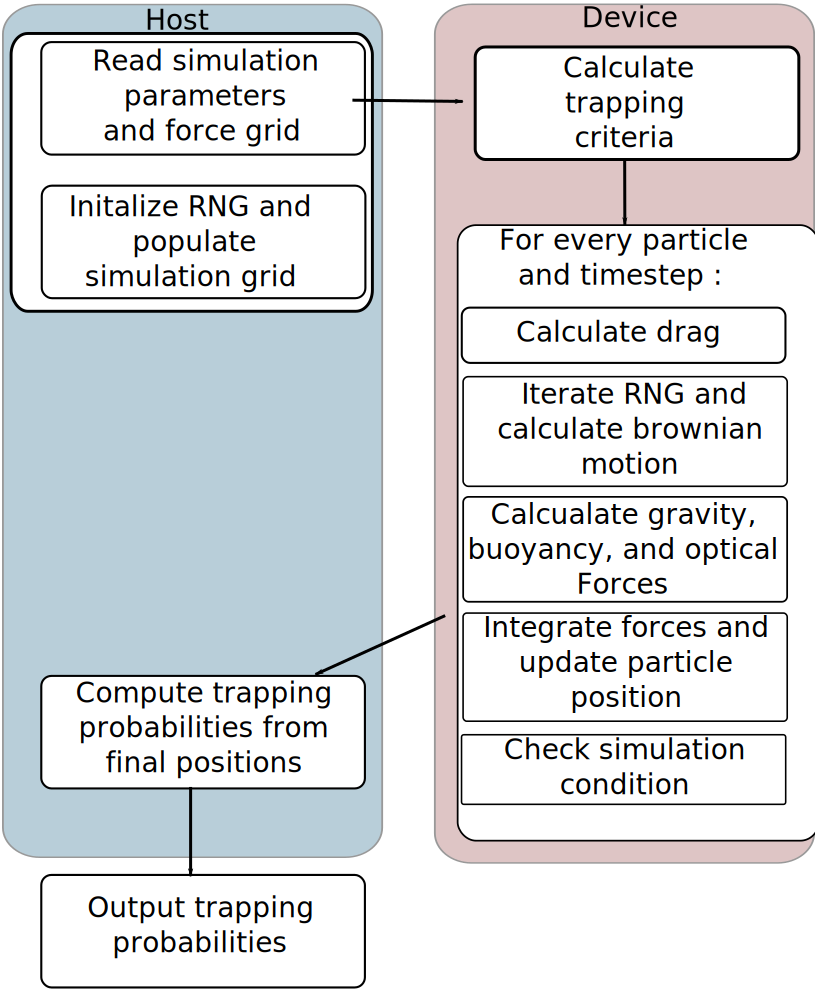
\includegraphics[width=\columnwidth]{figures/overview}
\caption{ An overview diagram of our system showing the distribution
  of work and the flow of data between the host and the device (GPU).
  Currently, the host is used only to load the initial simulation
  parameters and set the initial particle positions.  The device
  performs the simulation of the particle trajectories and returns the
  final positions to the host, which then simply computes the fraction
  of trapped particles corresponding to each initial position.  }
\label{fig:overview}
\end{figure}

%\documentclass{article}
%\begin{document}

With the experimental setup fully initialized, we are ready to perform
the massively parallel simulation of multiple particles on the GPU.
For a specific point $x_*$ in the workspace, we perform $N = 1024$
simulations in parallel.  Note that, for each individual simulation
run, the return value is a binomial random variable of 0 (not trapped)
or 1 (trapped); thus, for simulation sample sizes of at least $30$
runs, its outcome can be fit to a Gaussian curve with mean $\mu =
P_T$, the trapping probability, and variance $\sigma^2 = \frac{P_T (1
  - P_T)}{N}$ ~\cite{Hines:2003}.  For $N = 1024$, this yields a $95\%$ confidence
interval with maximum error of less than $\pm 0.03125$.


After initializing $N$ particles to the desired starting position 
$x_*$ and all active lasers to their initial positions and velocities, 
we assign each particle and laser to a thread on the GPU.  
We then execute Algorithm~\ref{alg:execution-main}.

\begin{algorithm}[t]
\caption{Parallel particle evolution on the GPU}
\label{alg:execution-main}

\begin{algorithmic}[1]
 \REQUIRE Set of active threads, each with pre-initialized particle $p$ and laser $l$ with velocity $v$. Time limit
$\textit{MAXTIME}$.
 \ENSURE Positions of particle and laser after $\textit{MAXTIME}$.

\FORALL{active threads (in parallel)}
  \WHILE{particle $p$ is not trapped and time $t < \textit{MAXTIME}$}
    \STATE calculate drag force\;
    \STATE calculate Brownian motion\;
    \STATE calculate sum of gravity, buoyancy, optical forces\;

    \IF{$\textit{trapped}(p, l, v)$}
      \STATE break\;
    \ENDIF

    \STATE second-order velocity Verlet integration to provide incremental update to velocity, position\;
    \STATE update position of laser $l$ according to velocity $v$\;
  \ENDWHILE

  \RETURN final positions of $p$ and $l$\;
\ENDFOR

\end{algorithmic}
\end{algorithm}

Algorithm~\ref{alg:execution-main} computes the final positions of each of the $N$ particles after some predetermined
period of time $\textit{MAXTIME}$.  The first loop (Line~1) executes in parallel on the GPU.  Line~3 calculates the
current drag force being applied to the particle.  As shown in Equation~\ref{eq:langevins-equation}, the drag force is
based on, among other things, a drag coefficient $\gamma$.  The value of $\gamma$ remains constant throughout the
simulation; as such, our implementation makes use of constant memory on the GPU to realize significant speedup. 
The nondeterministic Brownian force is calculated at Line~4 using the streaming GPU-specific random number generator
discussed in Section~\ref{sec:parallel-overview}.  Line~5 calculates a summation of forces, including the optical
force $F$ applied by the laser, through a combination of constant memory and texture memory.  Numerical evolution in
Line~9 updates the positions of the particles and lasers through velocity Verlet integration; this already quick method
is further sped up through GPU-specifc ``fast'' algebraic operations.

When Algorithm~\ref{alg:execution-main} returns, the host gathers all
$N$ final positions of particles $p_i$ for $i \in [1,N]$ and lasers
$l$. It then computes the set of {\em trapped} particles,
$\textit{TRAPPED}$, as follows:
\begin{equation}
\textit{TRAPPED} = \left\{ p_i | \textit{trapped}(p_i, l, v_l) \right\}
\end{equation}

In other words, the set of trapped particles, $\textit{TRAPPED}$, is the set of all particles, $p_{i}$, which, at the termination of the simulation, adhere to the trapping conditions of lasers $\ell_{j} \in l$ which are moving with corresponding velocities $v_{\ell_{j}}$.

From this, the probability (with 95\% confidence interval of $\pm 0.03125$) that a particle starting from location $x_*$
will be trapped by a laser with velocity $v_l$ within time period \textit{MAX\_TIME} is:
\begin{equation}
     P_T = \frac{\left|\textit{TRAPPED}\right|}{N}
\end{equation}

%\end{document}


%%%%%%%%%%%%%%%%%%%%%%%%%%%%%%%%%%%%%%%%%%%%%%%%%%%%%%%%%%%%%%%%%%%%%%
\section{Results}
\label{sec:results}

\subsection{Trapping Probabilities}
%%
%% res_trapping_probabilities.tex
%% 
%% Made by Robert Patro
%% Login   <rob@gvilwks03>
%% 
%% Started on  Tue Mar  9 13:18:45 2010 Robert Patro
%% Last update Tue Mar  9 13:18:45 2010 Robert Patro
%%

We evaluate the trapping probability for particles under the effect of
both a stationary and moving laser.  The trapping probabilities are
estimated on a discrete grid of positions relative to the focus of the
laser.  In all of our experiments, we consider a grid whose extents
match that of the discrete laser force grid $F$.  We sample this
grid in the $y$ and $z$ directions at a resolution of
$\SI{0.25}{\micro\meter}$.

\subsubsection{Trapping Probabilities under a Stationary Laser}

%Figures~\ref{fig:trapping-prob-static-gpu}
%and~\ref{fig:trapping-prob-static-cpu} illustrate how the probability
%of trapping a particle varies with respect to the particle's distance
%from the laser in both the $y$ and $z$ directions, under the influence
%of a stationary laser.  To verify the accuracy of our trapping
%probability estimates, we examine how the estimates computed using our
%GPU implementation differ from those computed using a CPU-based
%implementation of the same particle dynamics model.  Since the
%underlying governing equations are the same, and we perform a
%sufficient number of simulations (i.e. $1024$ per grid position) to
%ensure $95\%$ confidence in our probability estimate, we expect to see
%very little different between the two plots.  Indeed, an examination
%of Figures ~\ref{fig:trapping-prob-static-gpu}
%and~\ref{fig:trapping-prob-static-cpu} satisfies this expectation.

%We compute how the probability
%of trapping a particle varies with respect to the particle's distance
%from the laser in both the $y$ and $z$ directions, under the influence
%of a stationary laser. 
Figures~\ref{fig:trapping-prob-static-gpu} illustrates how the probability
of trapping a particle varies with respect to the particle's distance
from the laser in both the $y$ and $z$ directions, under the influence
of a stationary laser. To verify the accuracy of our trapping
probability estimates, we examine how the estimates computed using our
GPU implementation differ from those computed using a CPU-based
implementation of the same particle dynamics model. Since the
underlying governing equations are the same, and we perform a
sufficient number of simulations (i.e. $1024$ per grid position) to
ensure $95\%$ confidence in our probability estimate, we expect to see
very little difference between the two plots. Figure~\ref{fig:trapping-prob-static-cpu-gpu-error} 
shows the difference in probability estimates between the two implementations.
The average error between the CPU and the GPU implementation of the
probability estimate (computed using L2 norm) is $0.00091$.


\begin{figure}[htb!]
%%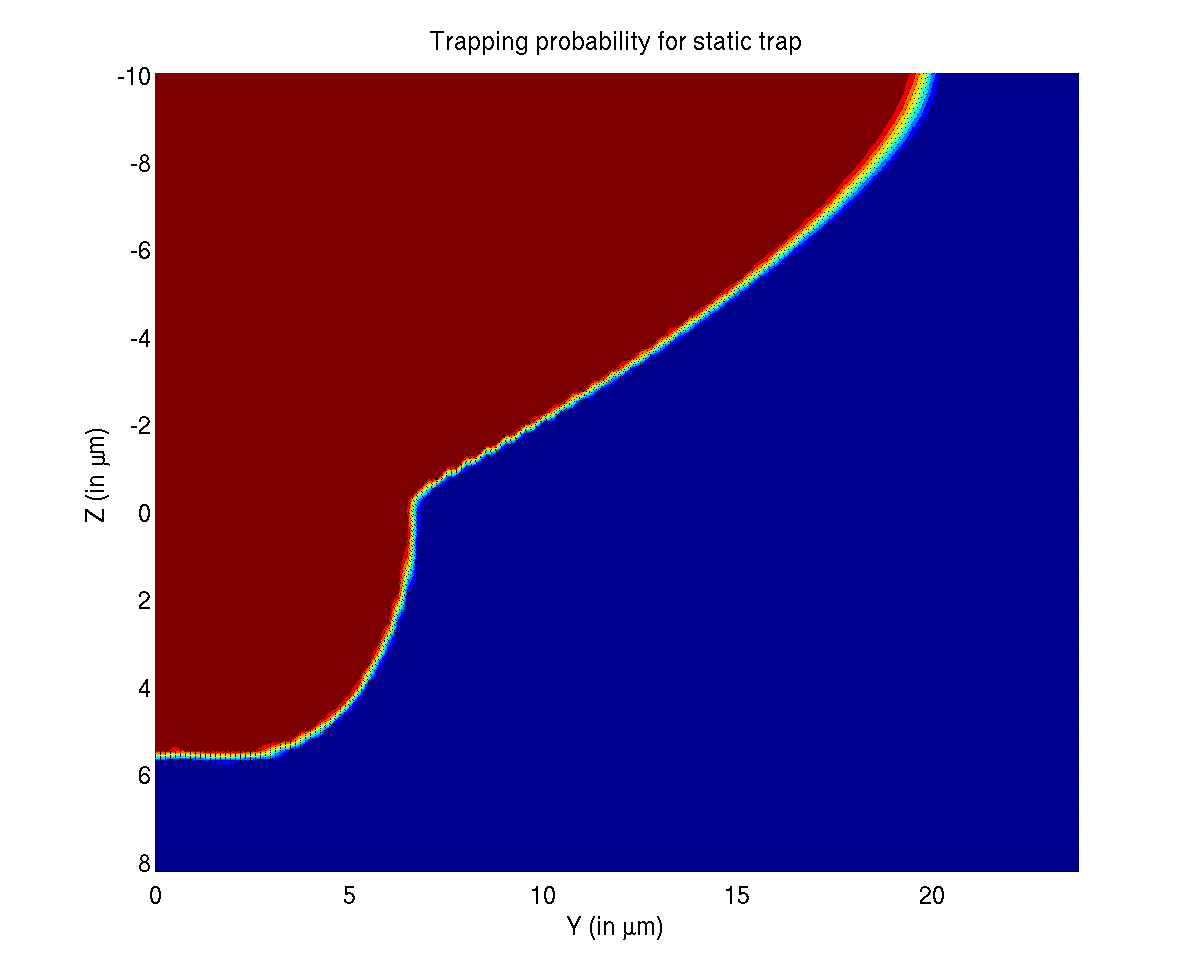
\includegraphics[width=\columnwidth]{figures/gpu_static_trap_prob_1_0s}
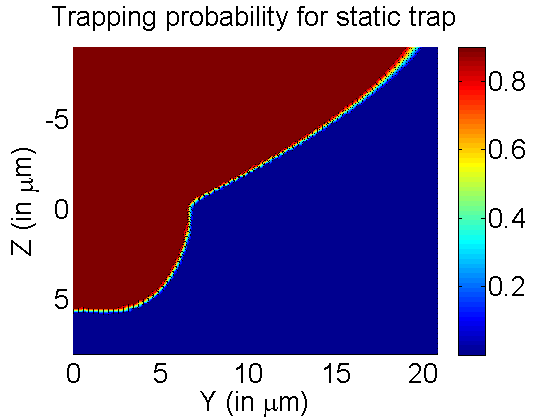
\includegraphics[width=\columnwidth]{figures/gpu_static_trap_prob_1024_particles}
\caption{This plot shows the probability of trapping a particle under
  the force exerted by a stationary laser with its focus at $(0,0)$,
  and was generated using the GPU implementation detailed in this paper.}
\label{fig:trapping-prob-static-gpu}
\end{figure}

%\begin{figure}[htb!]
%%%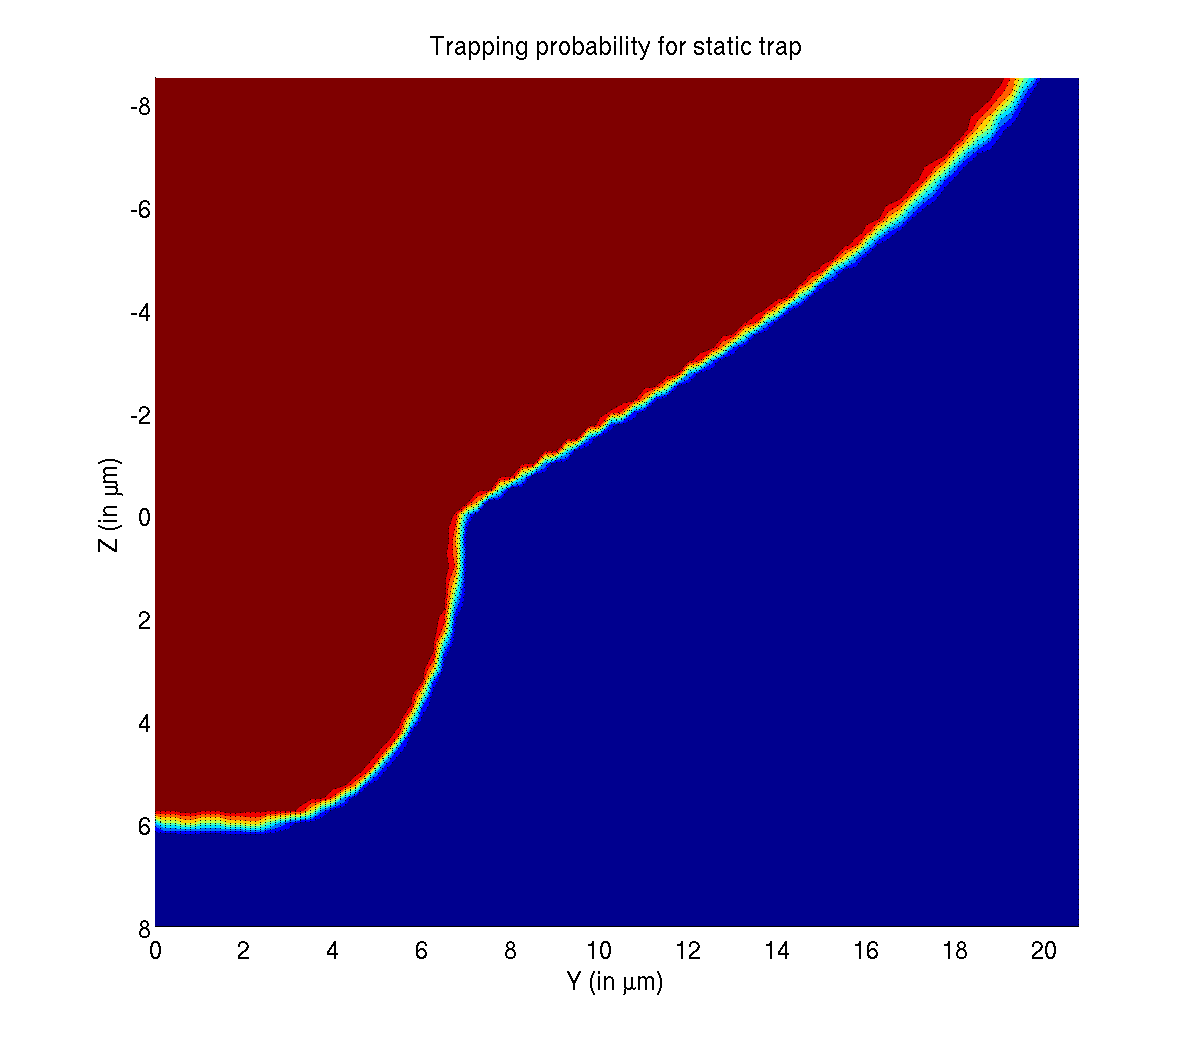
\includegraphics[width=\columnwidth]{figures/cpu_static_trap_prob_1_0s}
%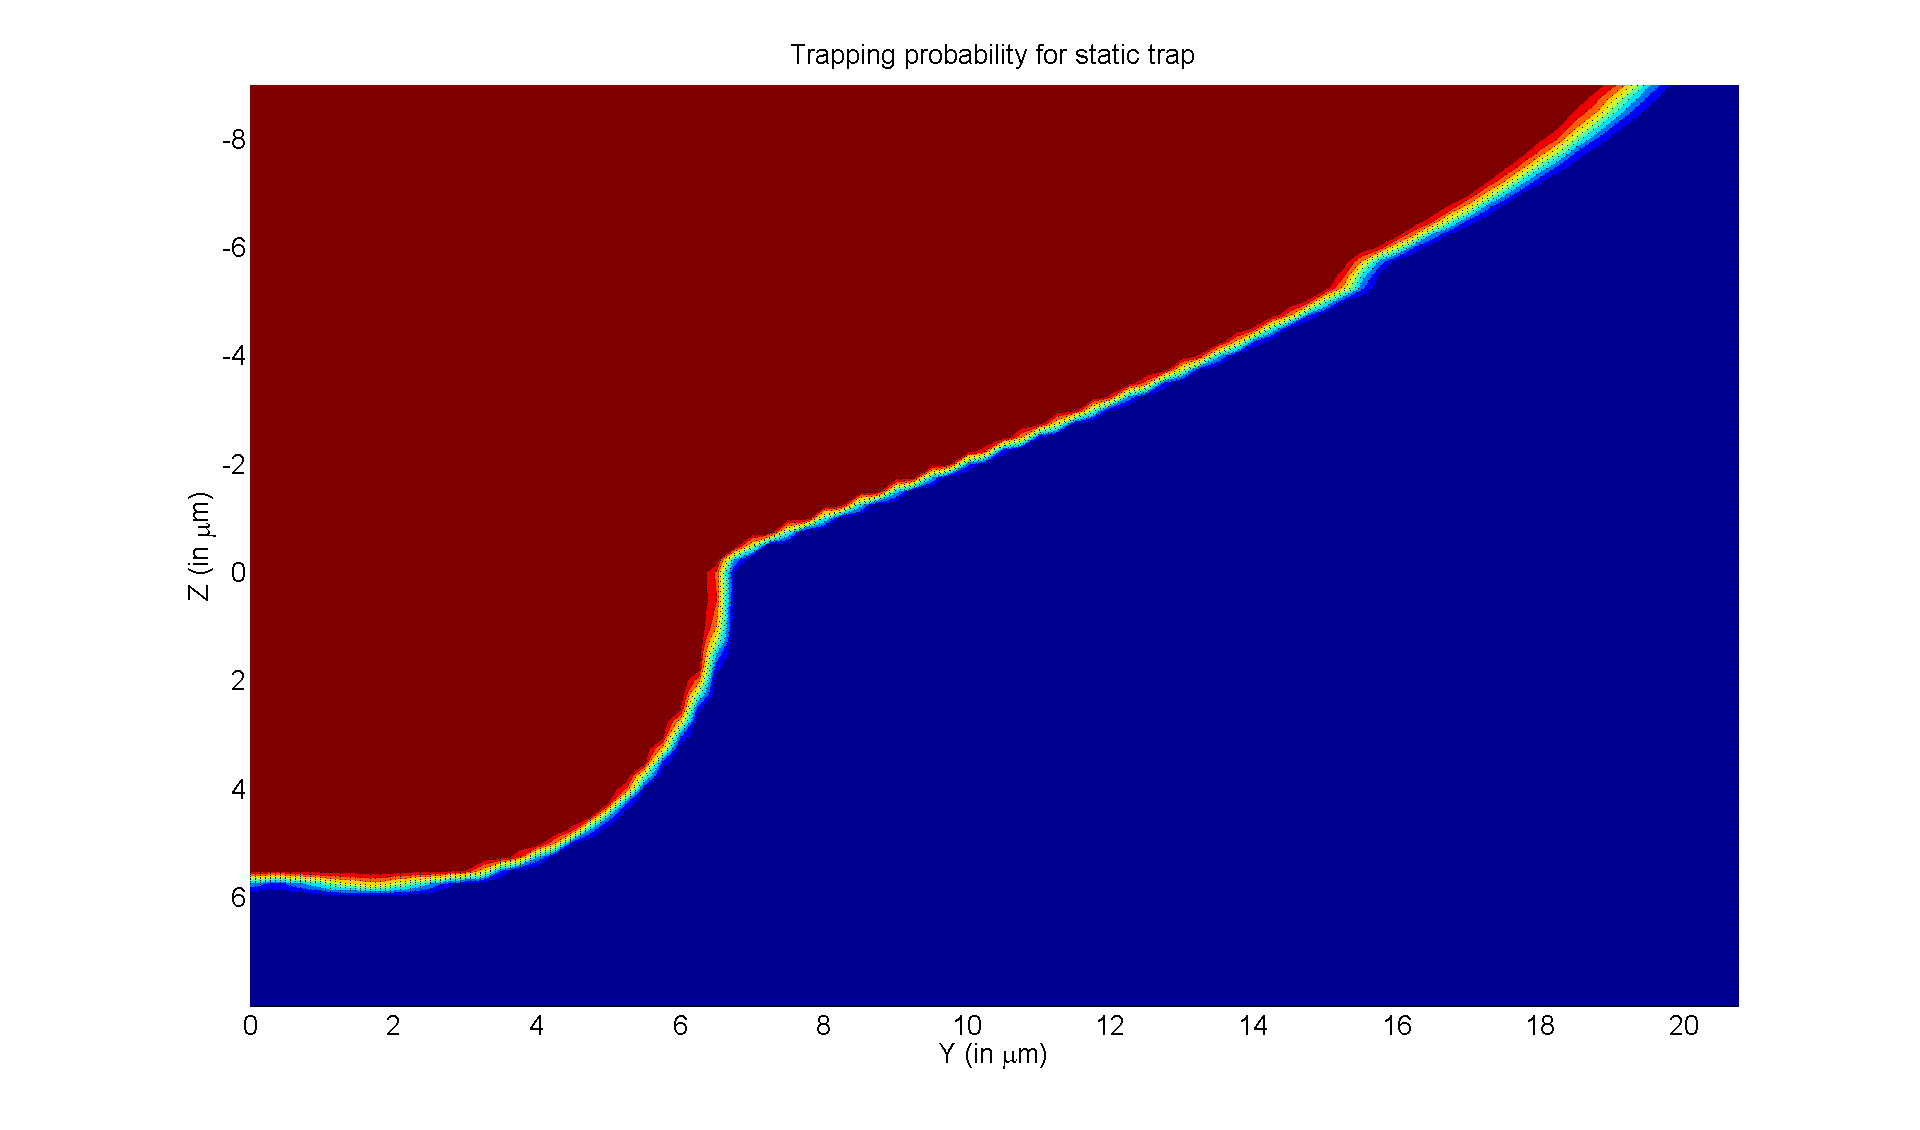
\includegraphics[width=\columnwidth]{figures/cpu_static_trap_prob_1024_particles}
%\caption{This plot shows the probability of trapping a particle under
%  the force exerted by a stationary laser with its focus at $(0,0)$.
%  This plot was generated using a CPU based implementation.}
%\label{fig:trapping-prob-static-cpu}
%\end{figure}

\begin{figure}[htb!]
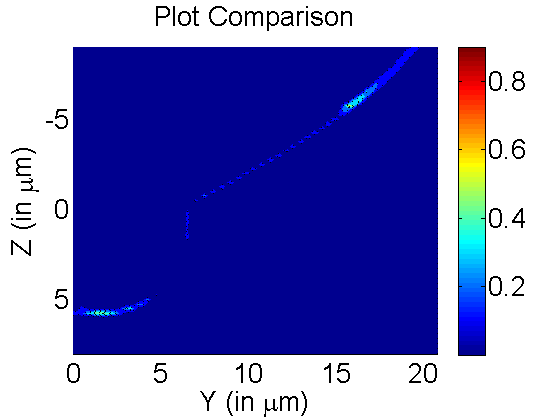
\includegraphics[width=\columnwidth]{figures/absolute_error}
\caption{
This plot shows the absolute difference between the CPU and the 
GPU implementation of the probability of trapping a particle under 
the force exerted by a stationary laser with its focus at $(0,0)$.
}
\label{fig:trapping-prob-static-cpu-gpu-error}
\end{figure}


We also examine the difference between probability estimates computed 
using single and double precision. We found the average error 
(computed using L2 norm) to be $ 0.00084$.


%\begin{figure}[htb!]
%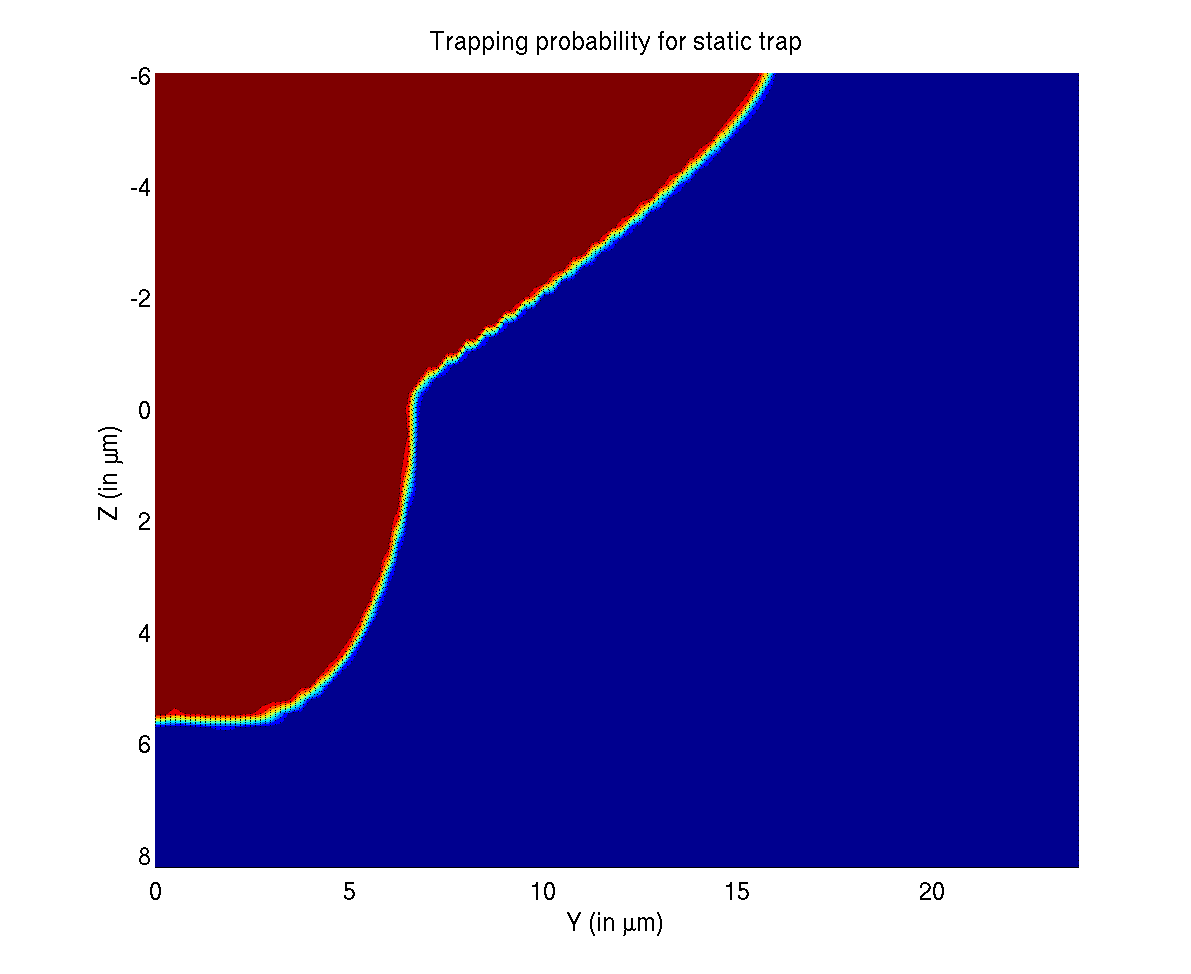
\includegraphics[width=\columnwidth]{figures/gpu_static_trap_prob_0_5s}
%\caption{This plot shows the probability of trapping a particle under
%  the force exerted by a stationary laser with its focus at $(0,0)$,
%  and was generated using the GPU implementation detailed in this
%  paper; the simulation duration was $0.5$s.}
%\label{fig:trapping-prob-static-gpu-0-5}
%\end{figure}
%
%
%\begin{figure}[htb!]
%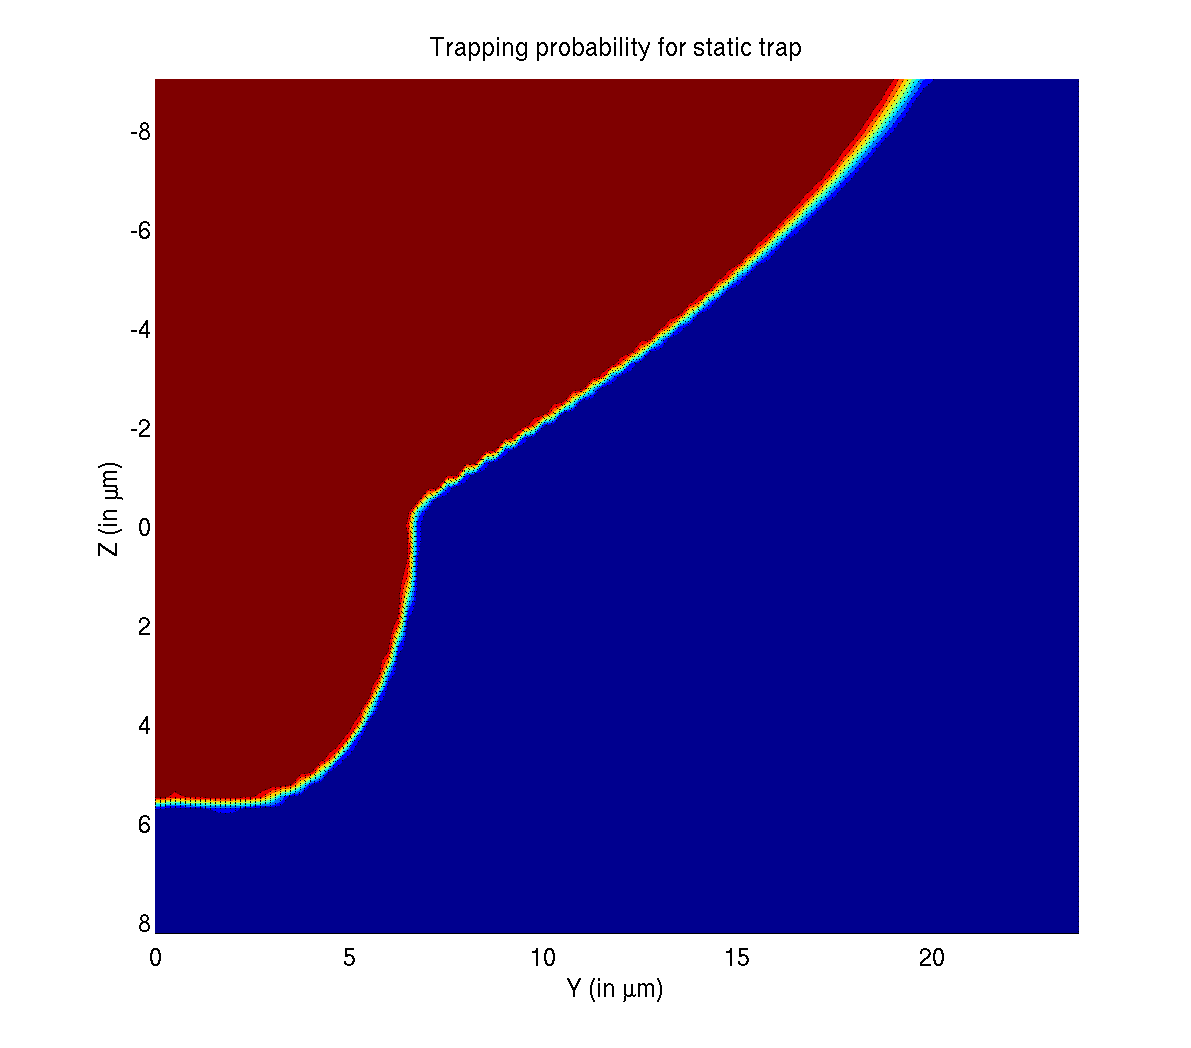
\includegraphics[width=\columnwidth]{figures/gpu_static_trap_prob_1_5s}
%\caption{This plot shows the probability of trapping a particle under
%  the force exerted by a stationary laser with its focus at $(0,0)$,
%  and was generated using the GPU implementation detailed in this
%  paper; the simulation duration was $1.5$s.}
%\label{fig:trapping-prob-static-gpu-1-5}
%\end{figure}
%
%\begin{figure}[htb!]
%%%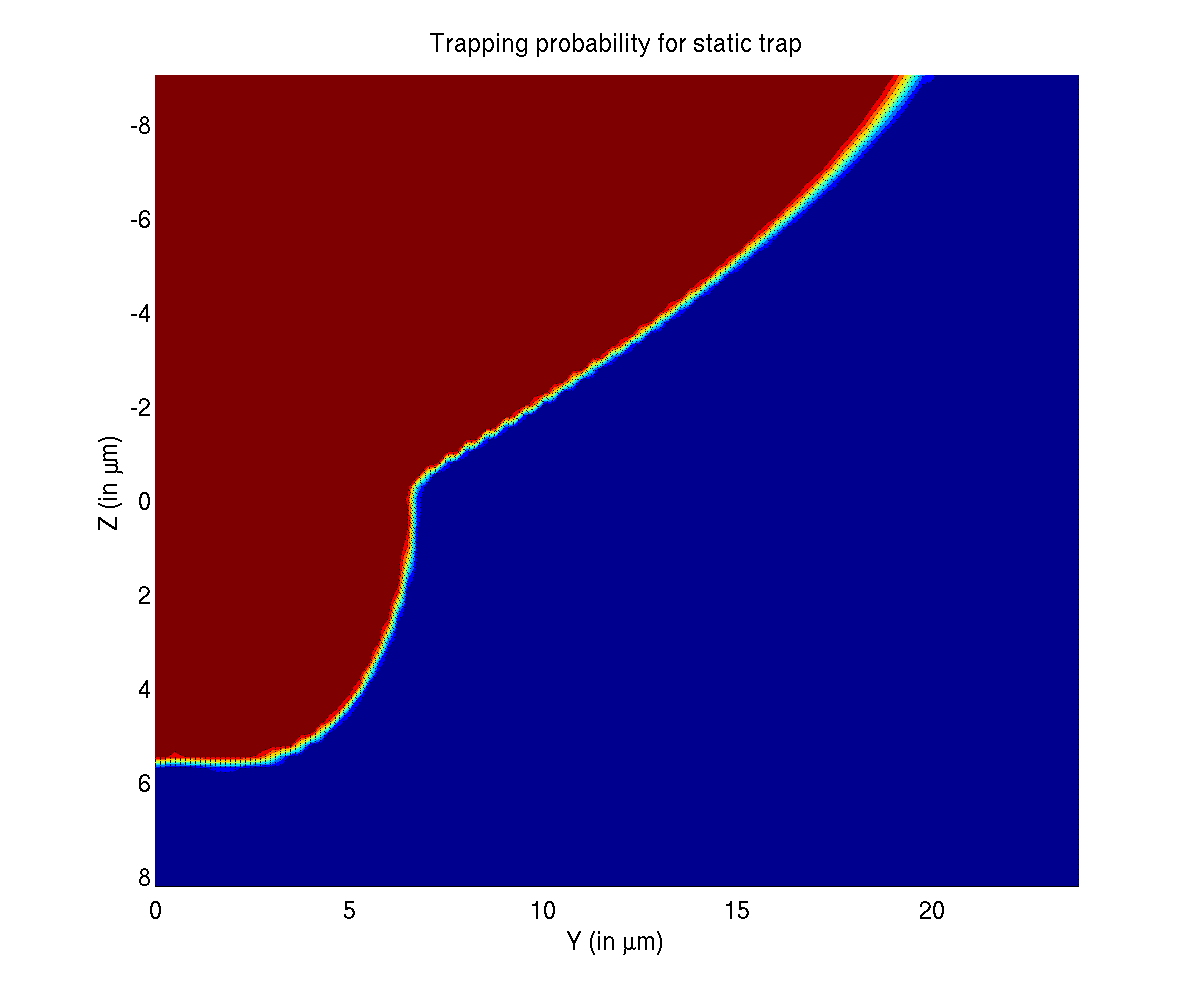
\includegraphics[width=\columnwidth]{figures/gpu_static_trap_prob_2_0s}
%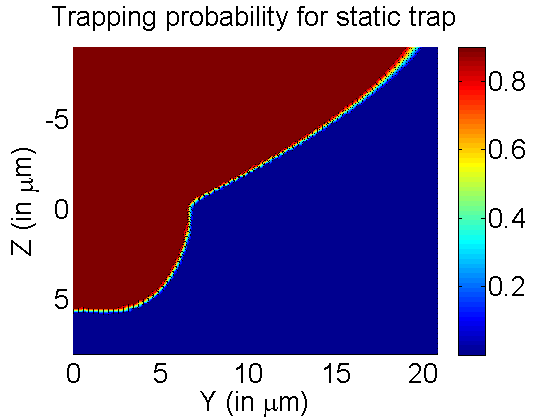
\includegraphics[width=\columnwidth]{figures/gpu_static_trap_prob_1024_particles}
%\caption{This plot shows the probability of trapping a particle under
%  the force exerted by a stationary laser with its focus at $(0,0)$,
%  and was generated using the GPU implementation detailed in this
%  paper; the simulation duration was $2.0$s.}
%\label{fig:trapping-prob-static-gpu-2-0}
%\end{figure}

\subsubsection{Trapping Probabilities under a Moving Laser}

Figures~\ref{fig:trapping-prob-xyvel-gpu}, and \ref{fig:trapping-prob-zvel-gpu}
%\ref{fig:trapping-prob-xyvel-cpu}, , and
%\ref{fig:trapping-prob-zvel-cpu} 
illustrate how the probability of
trapping a particle varies with respect to the particle's distance from
the laser in both the $y$ and $z$ directions, under the influence of a
moving laser.  In particular, we consider a laser moving with a
constant velocity of $\SI{0.65}{\micro\meter\per\milli\second}$
in the $y$ direction as well as a laser moving with a constant
velocity of $\SI{0.325}{\micro\meter\per\milli\second}$ in the
$z$ direction.

\begin{figure}[htb!]
  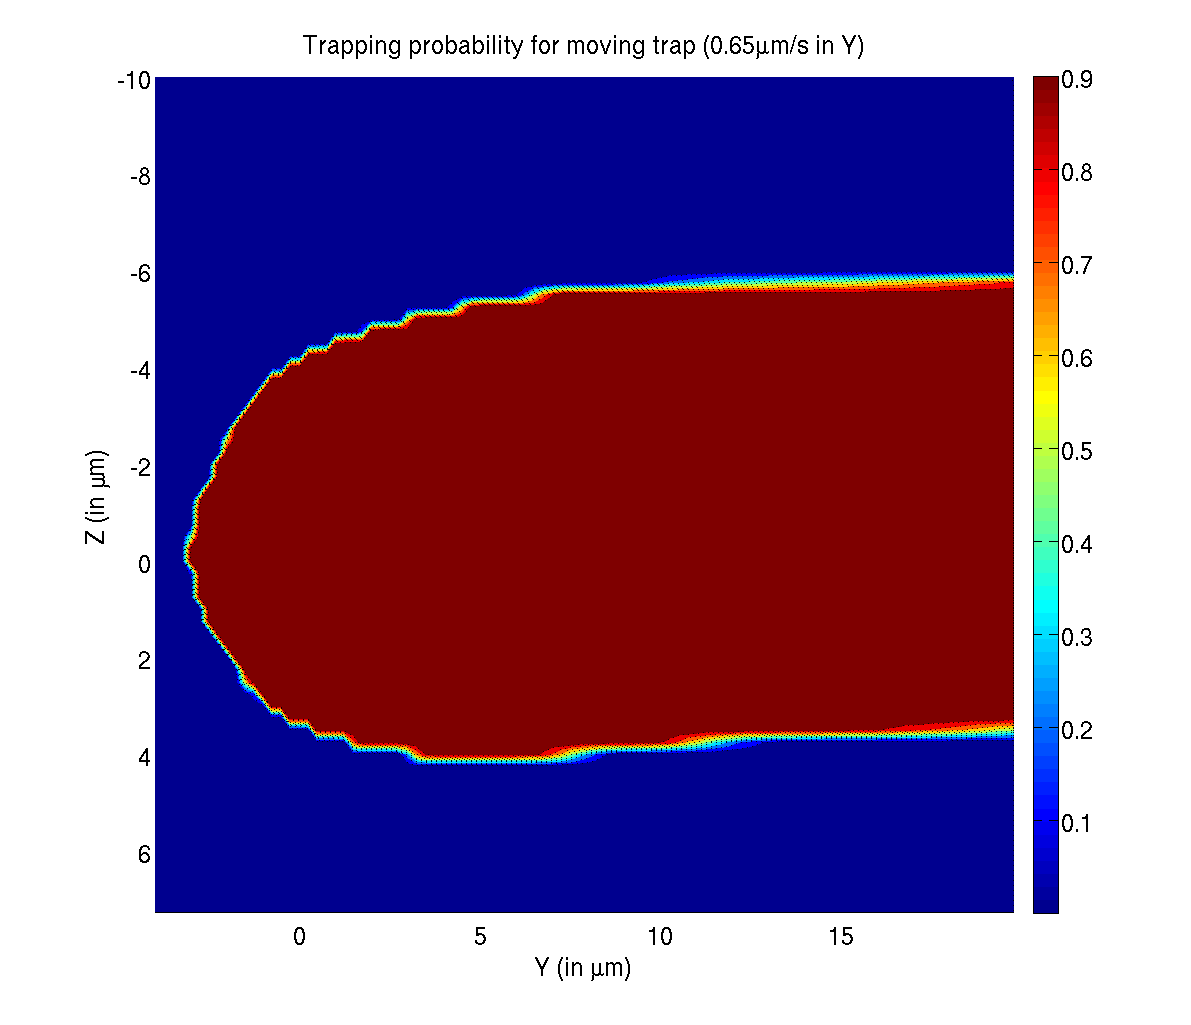
\includegraphics[width=\columnwidth]{figures/gpu_moving_0_65_y}
\caption{
  This plot shows the probability of trapping a particle under
  the force exerted by laser moving at a constant velocity of
  $\SI{0.65}{\micro\meter\per\milli\second}$ in the direction
  $(1,0)$, and was generated using the GPU implementation detailed in 
  this paper.
}

\label{fig:trapping-prob-xyvel-gpu}
\end{figure}


% \begin{figure}[htb!]
% \caption{
%   This plot shows the probability of trapping a particle under
%   the force exerted by laser moving at a constant velocity of
%   $\SI{0.65}{\frac{\micro\meter}{\milli\second}}$ in the direction
%   $(1,0)$, and was generated using a CPU-based implementation.
% }
% \label{fig:trapping-prob-xyvel-cpu}
% \end{figure}

\begin{figure}[htb!]
  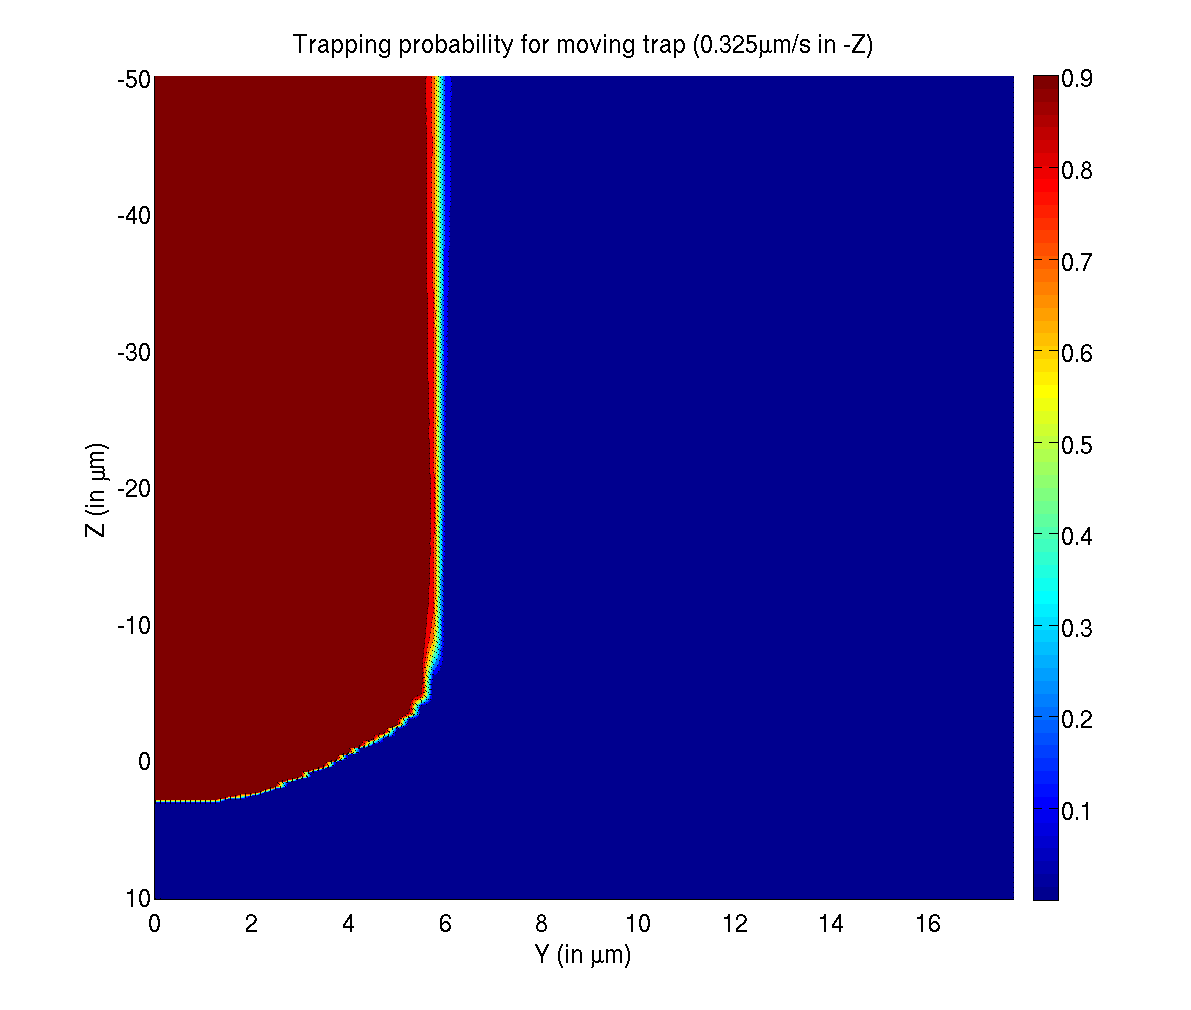
\includegraphics[width=\columnwidth]{figures/gpu_moving_0_325_z}
\caption{
  This plot shows the probability of trapping a particle under
  the force exerted by laser moving at a constant velocity of
  $\SI{0.325}{\micro\meter\per\milli\second}$ in the direction
  $(0,-1)$, and was generated using the GPU implementation detailed in 
  this paper.
}
\label{fig:trapping-prob-zvel-gpu}
\end{figure}

% \begin{figure}[htb!]

% \caption{
%   This plot shows the probability of trapping a particle under
%   the force exerted by laser moving at a constant velocity of
%   $\SI{0.325}{\frac{\micro\meter}{\milli\second}}$ in the direction
%   $(0,-1)$, and was generated using a CPU-based implementation.
% }
% \label{fig:trapping-prob-zvel-cpu}
% \end{figure}



%%% Local Variables: 
%%% mode: latex
%%% TeX-master: t
%%% End: 


\subsection{Timing}
To obtain a timing comparison between the CPU-based and GPU-based
simulations, we parametrize over the number of particles.  Given a
grid spacing of $0.25$ microns and a grid over $\left[0, 20\right]
\times \left[-20, +8\right]$, we must test $9744$ positions.  
%Assuming $100$ particles per position to achieve a confidence of 
%$\pm 0.1\%$, this results in roughly one million tests.
Assuming $1024$ particles per position to achieve a $95\%$ confidence
interval with maximum error of less than $\pm 0.03125$, this results 
in roughly ten million tests. The performance results
can be seen in Figure~\ref{fig:gpu-cpu-performance}.  As the number of
particles increases, so does the benefit of the GPU-based parallel
simulation.  At $N=4096$ particles per grid cell, the GPU-based
simulation is $\sim 356$ times faster than its CPU-based counterpart.


\begin{figure}
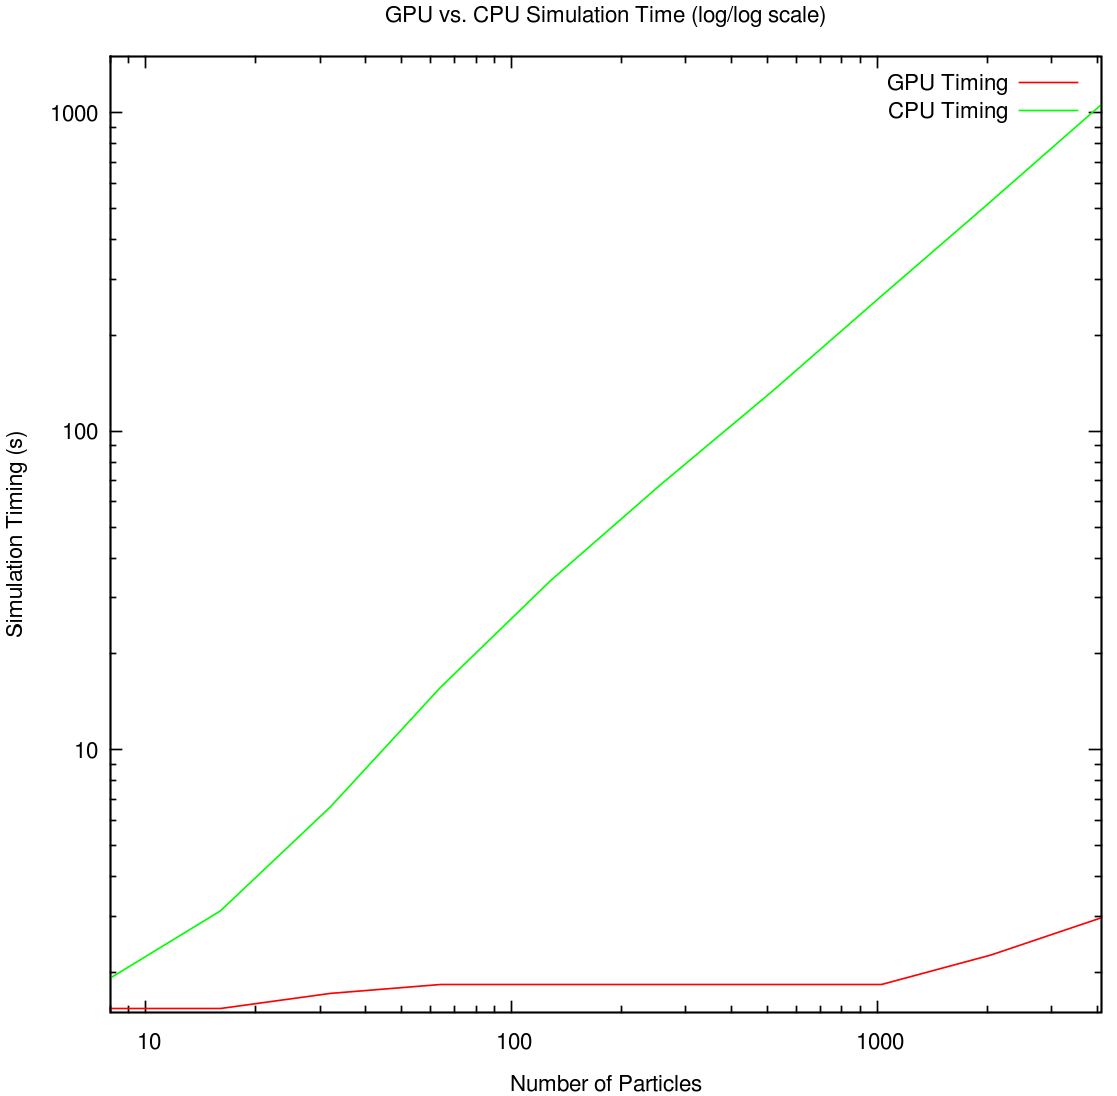
\includegraphics[width=\columnwidth]{figures/gpu_cpu_timings.png}
\caption{\label{fig:gpu-cpu-performance}The running time required as a
  function of the number of trajectories calculated using both the CPU
  and GPU simulators.  The plots have been placed on a log-log scale.
  The CPU simulator exhibits exactly the type of linear performance
  curve we expect, while GPU performance slowed by less than a factor
  of $2$ between $8$ and $4096$ trajectories.}
\end{figure}

%%%%%%%%%%%%%%%%%%%%%%%%%%%%%%%%%%%%%%%%%%%%%%%%%%%%%%%%%%%%%%%%%%%%%%
\section{Conclusion and Future Work}

We have introduced a GPU-based framework for massive simulation of particle
motion under user-defined force fields.  We applied this framework
experimentally to the well-studied problem of computing the trapping
probabilities associated with micron-sized silica beads in optical
trapping workbenches.  The simulator handles both stationary and
moving laser-induced force fields and, due to the highly parallel nature of the problem
and efficient use of the available hardware, exhibits a significant
speedup over its CPU-based analog. In particular, when evaluating many
trajectories ($4096$), we see approximately a $356$ times speedup of
the GPU based simulator over its CPU based counterpart.  This speedup
is more than can be accounted for by the increased processor count on
the GPU, and we attribute the extra performance to the higher memory
bandwidth, spatially coherent caching, and hardware accelerated
bilinear interpolation of the laser force field in the GPU simulator.
In particular, this last operation must be performed in software on
the CPU.  We believe this work indicates that GPUs hold great promise
in accelerating the type of compute-intensive simulations that are
required when working with optical tweezers and nanoscale assembly in
general.  Often times, the stochastic nature of such simulations leads
to a probabilistic approach involving many independent trials, a setup
whose parallelism uniquely suits the type of high-throughput
computation enabled by modern GPUs.

In the future, we are interested in extending this work to deal with
more general types of nanocomponents, perhaps even those which cannot
be defined analytically.  We are also interested in investigating
other areas of the optical workbench workflow where GPUs can be used
to accelerate computational bottlenecks in the process.


%\todo[inline]{Why our results are good}

%%%%%%%%%%%%%%%%%%%%%%%%%%%%%%%%%%%%%%%%%%%%%%%%%%%%%%%%%%%%%%%%%%%%%%
%\section{Future Work}
%\todo[inline]{Where we intend to take this work in the future}

%%%%%%%%%%%%%%%%%%%%%%%%%%%%%%%%%%%%%%%%%%%%%%%%%%%%%%%%%%%%%%%%%%%%%%
\begin{acknowledgment}
  This work has been supported in part by the NSF grants: CCF
  04-29753, CNS 04-03313, CCF 05-41120 and CMMI 08-35572. We also
  gratefully acknowledge the support provided by the NVIDIA CUDA
  Center of Excellence award to the University of Maryland and
  constructive discussions with David Luebke at NVIDIA research. Any
  opinions, findings, conclusions, or recommendations expressed in
  this article are those of the authors and do not necessarily reflect
  the views of the research sponsors.
\end{acknowledgment}

%%%%%%%%%%%%%%%%%%%%%%%%%%%%%%%%%%%%%%%%%%%%%%%%%%%%%%%%%%%%%%%%%%%%%%
% The bibliography is stored in an external database file
% in the BibTeX format (file_name.bib).  The bibliography is
% created by the following command and it will appear in this
% position in the document. You may, of course, create your
% own bibliography by using thebibliography environment as in
% \begin{thebibliography}{12}
% ...
% \bibitem{itemreference} D. E. Knudsen.
% {\em 1966 World Bnus Almanac.}
% {Permafrost Press, Novosibirsk.}
% ...
% \end{thebibliography}

% Here's where you specify the bibliography style file.
% The full file name for the bibliography style file 
% used for an ASME paper is asmems4.bst.
\bibliographystyle{asmems4}

% Here's where you specify the bibliography database file.
% The full file name of the bibliography database for this
% article is asme2e.bib. The name for your database is up
% to you.
\nocite{*}
\bibliography{gpu_tweezers}

\end{document}
